%% Springer Nature journal article (sn-jnl template, numbered references).
%% Uses the official sn-jnl.cls when present; otherwise falls back to the local
%% preview shim sn-jnl-compat.cls so that the draft can be compiled anywhere.
\IfFileExists{sn-jnl.cls}{%
  \documentclass[pdflatex,sn-mathphys-num]{sn-jnl}%
}{%
  \documentclass{sn-jnl-compat}%
}

\usepackage{graphicx}
\usepackage{multirow}
\usepackage{amsmath,amssymb,amsfonts}
\usepackage{amsthm}
\usepackage{mathrsfs}
\usepackage[title]{appendix}
\usepackage{xcolor}
\usepackage{textcomp}
\usepackage{manyfoot}
\usepackage{booktabs}
\usepackage{rotating}
\usepackage{siunitx}
\sisetup{range-phrase=--, separate-uncertainty=true}
\DeclareSIUnit\molar{M}
\makeatletter\newcommand{\inputtable}[1]{\@@input #1 }\makeatother
\graphicspath{{figures/}}

\raggedbottom

\begin{document}

\title[Bioimpedance and electrochemistry of CAP-treated infected wound phantoms]{Wideband Bioimpedance and Electrochemical Characterization of Cold Atmospheric Plasma-Treated Infected Wound Phantoms: A Multiphysics In Silico Study}

\author*[1]{\fnm{M.} \sur{Nisha Angeline}}\email{nishavlsidesign@gmail.com}

\affil*[1]{\orgdiv{Department of Electronics and Communication Engineering}, \orgname{Velalar College of Engineering and Technology}, \orgaddress{\street{Thindal}, \city{Erode}, \postcode{638012}, \state{Tamil Nadu}, \country{India}}}

\abstract{\textbf{Purpose:} Cold atmospheric plasma (CAP) is a non-antibiotic option for infected chronic wounds, but its antimicrobial dose is still verified by destructive colony counting. We asked whether wideband bioimpedance and electrochemical read-outs can report CAP efficacy label-free, and which spectral features carry the information.
\textbf{Methods:} We built an open, reproducible multiphysics framework for a layered wound phantom (\SI{100}{\micro\metre} \textit{Staphylococcus aureus} biofilm on a \SI{3}{\milli\metre} phosphate-buffered agarose wound bed). It couples (i) depth-resolved diffusion--reaction of plasma-derived H$_2$O$_2$, NO$_2^-$, NO$_3^-$ and H$^+$ with bacterial catalase scavenging, (ii) Weibull inactivation and membrane permeabilisation, (iii) single-shell/Maxwell--Garnett dielectric modelling of the biofilm read by an interdigitated electrode from \SI{10}{\hertz} to \SI{100}{\mega\hertz}, and (iv) screen-printed-electrode electrochemistry (Faradaic impedance, finite-difference cyclic voltammetry, Prussian-blue H$_2$O$_2$ amperometry and IrO$_x$ pH sensing). Fifty-four virtual phantoms (nine groups, $n=6$, including Ar-gas-only and sterile controls) with realistic phantom-to-phantom variability and instrument noise were analysed by complex non-linear least squares, Lin-KK validation, ANOVA/Tukey tests and nested partial-least-squares regression.
\textbf{Results:} All spectra passed the Kramers--Kronig test (RMS residual 0.28\%). CAP exposure of 30--300\,s produced 0.31--2.11 log$_{10}$ reductions. The biofilm $\beta$-dispersion decreased from $\Delta\varepsilon = 182\pm10$ to $78\pm2$ and its characteristic frequency rose from 16.6 to 27.1\,MHz; $f_c$ was the most discriminating feature ($\eta^2=0.973$, Spearman $\rho=-0.95$ against viable count) and kept separating 180 from 300\,s after $\Delta\varepsilon$ saturated. Charge-transfer resistance fell by 40\% as the biofilm blocked less of the electrode. Ar gas alone changed no read-out, whereas sterile phantoms showed a 5\% ionic/evaporative conductivity artefact and a 16-fold higher H$_2$O$_2$ load than infected ones. A nested-cross-validated PLS model predicted viable counts from raw spectra with RMSECV = 0.52 log.
\textbf{Conclusion:} Within the model, the high-MHz $\beta$-dispersion is a label-free marker of CAP-induced membrane damage, and an electrochemical channel adds a direct reading of the delivered H$_2$O$_2$. The framework sets out the frequencies, controls and sensitivity bounds for planned wet-laboratory validation. All results here are simulated.}

\keywords{Cold atmospheric plasma, Bioimpedance spectroscopy, Electrochemical impedance spectroscopy, Wound phantom, Biofilm, Maxwell--Wagner dispersion, Reactive oxygen and nitrogen species}

\maketitle

%% ===================================================================
\section{Introduction}\label{sec:intro}

Chronic wounds such as diabetic foot and venous leg ulcers are often colonised by polymicrobial biofilms that tolerate antibiotics and antiseptics. Cold atmospheric plasma (CAP), a partially ionised gas near room temperature, delivers a mixture of short- and long-lived reactive oxygen and nitrogen species (RONS), ultraviolet photons and electric fields to the wound surface \cite{graves2012,lu2016,vonwoedtke2019}. In a randomised controlled trial, daily 5-min treatments with an argon plasma reduced bacterial load in chronic wounds by 34\% \cite{isbary2010}. Reviews of animal and clinical work report antimicrobial, pro-angiogenic and immunomodulatory effects \cite{bekeschus2021,raissi2025,moszczynska2023}. Laboratory results nonetheless vary widely. Biofilms of \textit{Staphylococcus aureus} and \textit{Pseudomonas aeruginosa} show strain-dependent tolerance \cite{baz2023}. Reductions on ex vivo human skin are often about one log after 5\,min \cite{bagheri2023}. In wet or deep environments, efficacy collapses once the liquid film is thicker than a few hundred micrometres \cite{hafner2018,plattfaut2021}. These differences reflect transport: plasma-generated species must cross the liquid--tissue interface and penetrate millimetre-scale tissue models before they reach the target cells \cite{szili2018}. Device geometry, gas chemistry and treatment mode also differ between laboratories, which makes results hard to compare \cite{maiprochnow2014,oconnor2014,nguyen2018}.

A practical obstacle in all of these studies is the read-out. Antimicrobial efficacy is measured by colony counting or live/dead staining, which destroys the sample, takes about a day and gives no spatial or temporal resolution. Electrical methods have been proposed as real-time, label-free alternatives. Impedance biosensors follow biofilm growth and dispersal \cite{mcglennen2023,kumar2023}. Electrochemical impedance and voltammetry on porous electrodes report biofilm coverage \cite{oconnorf2025}. Machine-learning analysis of impedance spectra has been used to estimate biofilm-covered area \cite{xu2019}. Dielectric spectroscopy of cell suspensions is well understood: the radiofrequency $\beta$-dispersion arises from interfacial (Maxwell--Wagner) polarisation of intact plasma membranes and collapses when the membranes are permeabilised \cite{asami2002,markx1999,grimes2015}. Tissue dielectric spectra are well described by Cole--Cole parametric models \cite{cole1941,gabriel1996b,gabriel1996c}. A CAP-damaged biofilm should therefore show a measurable change in its $\beta$-dispersion. To our knowledge, this hypothesis has not been tested quantitatively in an infected wound model where plasma chemistry, depth-dependent killing, ionic artefacts and electrode effects all act together.

We address this question with a multiphysics in silico study. Its purpose is to design and de-risk a wet-laboratory campaign, not to replace one. The contributions are:
\begin{enumerate}
\item an open framework that links CAP surface fluxes to RONS profiles, depth-resolved inactivation and membrane permeabilisation in a layered biofilm/hydrogel wound phantom;
\item physically based forward models of an interdigitated-electrode (IDE) bioimpedance measurement from \SI{10}{\hertz} to \SI{100}{\mega\hertz} and of a screen-printed carbon electrode (SPCE) electrochemical suite (Faradaic EIS, cyclic voltammetry, H$_2$O$_2$ amperometry and pH potentiometry);
\item a statistically designed virtual experiment ($n=6$ per group, nine groups) with gas-only and sterile controls that separate biological from ionic and evaporative effects;
\item a ranking of spectral features and frequencies, a cross-validated chemometric predictor of viable count, and a sensitivity analysis that sets the requirements for experimental validation.
\end{enumerate}

%% ===================================================================
\section{Methods}\label{sec:methods}

\subsection{Phantom and treatment model}\label{sec:phantom}

Figure~\ref{fig:schematic} shows the virtual phantom. A \SI{3}{\milli\metre} agarose wound bed is prepared in simulated wound fluid with \SI{10}{\milli\molar} phosphate buffer (pH 7.4) and a conductivity of $\sigma_g = \SI{1.0}{\siemens\per\metre}$ at \SI{25}{\celsius}. It carries a \SI{100}{\micro\metre} \textit{S.~aureus} biofilm with a cell volume fraction $\phi = 0.30$ and an initial load of $10^{8}$\,CFU\,cm$^{-2}$. An argon plasma jet treats the surface for $t_{\mathrm{CAP}} \in \{30, 60, 120, 180, 300\}$\,s. Each treatment is followed by a 10-min hold before measurement. The jet is represented by constant surface fluxes $\Gamma_{\mathrm{H_2O_2}} = 2.0$, $\Gamma_{\mathrm{NO_2^-}} = 1.1$ and $\Gamma_{\mathrm{NO_3^-}} = 0.7$\,\si{\micro\mol\per\square\metre\per\second}, and a proton flux equal to the total acid flux. These values give column-mean concentrations of tens to about one hundred micromolar after 5\,min (Fig.~\ref{fig:chem}a), which is the order typically reported for kHz Ar jets \cite{lu2016,bagheri2023}. Species transport obeys
\begin{equation}
\frac{\partial c_i}{\partial t} = \frac{\partial}{\partial z}\!\left(D_i h(z) \frac{\partial c_i}{\partial z}\right) - k_{\mathrm{cat}}\, \nu(z)\, \delta_{i,\mathrm{H_2O_2}}\, c_i,
\qquad -D_i h \frac{\partial c_i}{\partial z}\Big|_{z=0} = \Gamma_i(t),
\label{eq:transport}
\end{equation}
where $h=0.45$ (biofilm) or $0.92$ (gel) is the hindrance factor, $\nu$ is the local viable density and $k_{\mathrm{cat}}=\SI{0.035}{\per\second}$ is the catalase-mediated consumption of H$_2$O$_2$ by an intact biofilm. Equation~\eqref{eq:transport} is solved on a non-uniform finite-volume grid (40 biofilm and 120 gel nodes) with an implicit scheme and $\Delta t=\SI{1}{\second}$. Mass is conserved to machine precision (Sect.~\ref{sec:verification}). The pH follows from the proton balance of the phosphate buffer ($\mathrm{p}K_a=7.2$). Conductivity changes are computed from limiting ionic conductivities, including the conductivity lost when HPO$_4^{2-}$ is protonated to H$_2$PO$_4^-$. Water lost to evaporation under the gas flow (\SI{0.4}{\micro\metre\per\second}) concentrates the electrolyte in both the plasma and the gas-only groups.

\begin{figure*}[t]
\centering
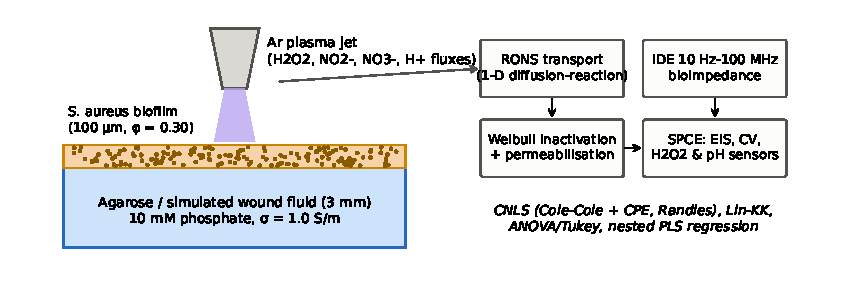
\includegraphics[width=\textwidth]{fig1_schematic}
\caption{Virtual infected wound phantom and analysis chain. A plasma jet imposes RONS fluxes on a \textit{S.~aureus} biofilm resting on a buffered agarose wound bed. Transport, inactivation and permeabilisation feed two measurement channels: a flexible interdigitated electrode (IDE) for \SIrange{10}{1e8}{\hertz} bioimpedance and a screen-printed carbon electrode (SPCE) for electrochemistry. Both are analysed by CNLS fitting, Kramers--Kronig validation and multivariate statistics.}
\label{fig:schematic}
\end{figure*}

\subsection{Inactivation and permeabilisation}

The local lethal dose combines H$_2$O$_2$ with the more toxic undissociated nitrous acid,
\begin{equation}
D(z) = \int_0^{t_{\mathrm{end}}} c_{\mathrm{H_2O_2}}\, \mathrm{d}t + w_{\mathrm{HNO_2}}\, f_{\mathrm{HNO_2}}(\mathrm{pH}) \int_0^{t_{\mathrm{end}}} c_{\mathrm{NO_2^-}}\, \mathrm{d}t,
\end{equation}
with $f_{\mathrm{HNO_2}} = [1+10^{\mathrm{pH}-3.4}]^{-1}$ and $w_{\mathrm{HNO_2}}=60$. Survival follows the Weibull (Mafart) model \cite{mafart2002}, $\log_{10} N/N_0 = -(D/\delta)^p$, with $\delta=\SI{60}{\milli\molar\second}$ and $p=0.85$; $p<1$ reproduces the tailing typical of biofilms. Membrane permeabilisation, the quantity that dielectric spectroscopy detects, is taken as the non-culturable fraction, $P(z) = 1 - N/N_0$. The biofilm-averaged log reduction is $-\log_{10}\langle N/N_0\rangle_z$. Exposure to the gas flow alone causes a desiccation stress of 0.04 log per 300\,s. The plasma jet also thins the biofilm at \SI{0.04}{\micro\metre\per\second}, through EPS etching and collapse of dead cells.

\subsection{Dielectric model of the biofilm}

Each coccus (radius $a=\SI{0.45}{\micro\metre}$) is a single-shell sphere with envelope thickness $d=\SI{6}{\nano\metre}$, $\varepsilon_m=6$ and $\sigma_m=\SI{e-7}{\siemens\per\metre}$, and cytoplasm with $\varepsilon_c=60$ and $\sigma_c=\SI{0.55}{\siemens\per\metre}$ \cite{asami2002,markx1999}:
\begin{equation}
\varepsilon_p^* = \varepsilon_m^* \frac{2(1-v)\varepsilon_m^* + (1+2v)\varepsilon_c^*}{(2+v)\varepsilon_m^* + (1-v)\varepsilon_c^*}, \qquad v = (1-d/a)^3,
\end{equation}
where $\varepsilon^* = \varepsilon' - j\sigma/(\omega\varepsilon_0)$. In a permeabilised cell the envelope conductivity rises to \SI{2e-3}{\siemens\per\metre}, the cytoplasm equilibrates halfway towards the extracellular conductivity and the radius shrinks by 10\%, in line with the deflation seen by electron microscopy after CAP \cite{baz2023}. Intact and permeabilised cells are mixed in the exopolysaccharide (EPS) matrix ($\sigma_{\mathrm{EPS}} = 0.85\,\sigma_g$) using the generalised Maxwell--Garnett rule,
\begin{equation}
\varepsilon_{\mathrm{bio}}^* = \varepsilon_h^*\, \frac{1+2S}{1-S}, \qquad S = \sum_k \phi_k \frac{\varepsilon_k^* - \varepsilon_h^*}{\varepsilon_k^* + 2\varepsilon_h^*}.
\end{equation}
The gel is described by a Debye water term plus its dc conductivity.

\subsection{Bioimpedance measurement model}\label{sec:ide}

A flexible gold IDE is pressed onto the biofilm. The electrode has cell constant $K=\SI{600}{\per\metre}$ (KCl-calibrated, with a 1\% replicate-to-replicate repositioning error), a field penetration length of $\lambda=\SI{45}{\micro\metre}$ \cite{igreja2004}, electrode polarisation (EP) represented by a constant-phase element (CPE; $Q=\SI{4e-7}{\siemens\second\tothe{n}}$, $n=0.82$) and \SI{1.5}{\pico\farad} of residual stray capacitance. Because the IDE sensitivity decays exponentially with height, the biofilm and the gel act as parallel paths:
\begin{equation}
Z(\omega) = \frac{1}{Q (j\omega)^n} + \left[\frac{j\omega\varepsilon_0}{K}\big(w_b \varepsilon_{\mathrm{bio}}^* + (1-w_b)\varepsilon_{\mathrm{gel}}^*\big) + j\omega C_s\right]^{-1}, \quad w_b = 1-e^{-d_b/\lambda}.
\label{eq:ide}
\end{equation}
Spectra are sampled at 141 log-spaced frequencies (20 per decade) from \SI{10}{\hertz} to \SI{100}{\mega\hertz}, matching the range of commercial impedance analysers. Each point carries proportional (0.25\%) plus additive (\SI{0.02}{\ohm}) complex Gaussian noise.

\paragraph{Parameter extraction.} Each spectrum is fitted by modulus-weighted complex non-linear least squares (CNLS; trust-region reflective, six starting points) to a seven-parameter model: an EP-CPE in series with a Cole--Cole dispersion and a dc conductivity \cite{cole1941},
\begin{equation}
\varepsilon^*(\omega) = \varepsilon_\infty + \frac{\Delta\varepsilon}{1+(j\omega/2\pi f_c)^{1-\alpha}} - j\frac{\sigma}{\omega\varepsilon_0}.
\end{equation}
The fit uses the nominal $K$, so repositioning error appears as replicate scatter. $\varepsilon_\infty$ also absorbs the stray capacitance. Standard errors are obtained from the Jacobian. Data quality is checked with the linear Kramers--Kronig test (Lin-KK) and automatic selection of the number of Voigt elements ($\mu<0.85$) \cite{schonleber2014}.

\subsection{Electrochemical measurement model}

Electrochemical phantoms are doped with \SI{5}{\milli\molar} equimolar [Fe(CN)$_6$]$^{3-/4-}$ and probed with a \SI{3}{\milli\metre} carbon SPCE. The biofilm blocks a fraction $\theta = \theta_0 (d_b/d_{b,0})(1 - 0.3P)$ of the electrode, with $\theta_0=0.62$ for an untreated biofilm and $0.03$ for the conditioning film on sterile phantoms. Blocking lowers the effective rate constant, $k^0_{\mathrm{eff}} = k^0(1-\theta)$ with $k^0 = \SI{2e-5}{\metre\per\second}$ (6\% replicate scatter), and the double-layer capacitance. The Faradaic impedance is the Randles circuit with a CPE and a semi-infinite Warburg element \cite{bard2001,orazem2008,brug1984}:
\begin{equation}
Z = R_s + \left[Q_{dl}(j\omega)^{n_{dl}} + \frac{1}{R_{ct} + \sigma_W(1-j)\omega^{-1/2}}\right]^{-1}, \quad R_{ct} = \frac{RT}{F^2 A k^0_{\mathrm{eff}} c^{*}}.
\end{equation}
It is sampled from \SI{0.1}{\hertz} to \SI{100}{\kilo\hertz} with 0.4\% noise. Cyclic voltammograms (\num{-0.2} to \SI{0.6}{\volt}, \SI{50}{\milli\volt\per\second}, second cycle reported) are obtained by explicit finite differences with Butler--Volmer boundary kinetics, iR drop and double-layer charging. A Prussian-blue-modified SPCE (sensitivity \SI{0.55}{\ampere\per\molar\per\square\centi\metre}, \SI{4}{\nano\ampere} noise) reads H$_2$O$_2$ in the biofilm layer. An IrO$_x$ micro-sensor (\SI{-58}{\milli\volt} per pH, \SI{1.5}{\milli\volt} noise) reads the surface pH.

\subsection{Virtual experimental design and statistics}

There are nine groups with six phantoms each ($N=54$): untreated Control; CAP-30, -60, -120, -180 and -300; Gas-300 (Ar flow, plasma off); Sterile; and Sterile+CAP-300. For each replicate, the following quantities are drawn independently: initial load ($8.0\pm0.15$ log), biofilm thickness ($100\pm\SI{8}{\micro\metre}$), cell fraction ($0.30\pm0.02$), gel conductivity ($\pm3\%$), plasma flux (log-normal, 10\%), susceptibility $\delta$ (log-normal, 12\%), EP parameters ($\pm5\%$), $K$ ($\pm1\%$) and $k^0$ (6\%). Group effects in the seven infected groups were tested by one-way ANOVA (effect size $\eta^2$) with Tukey HSD post hoc comparisons. Sterile groups were compared by Welch's $t$-test. Monotonic associations with viable count were quantified by Spearman's $\rho$. Raw spectra (log$|Z|$ and phase, 282 variables) were regressed on log$_{10}$ CFU by partial least squares (PLS) \cite{wold2001} in a nested scheme: leave-one-out outer loop, 5-fold inner loop for the number of latent variables. Variable-importance-in-projection (VIP) scores identified the informative bands. One-at-a-time $\pm20\%$ perturbations of eight model inputs quantified how robust the main bioimpedance contrast is. The full study runs in under one minute on a laptop (Python 3.13, NumPy, SciPy \cite{virtanen2020}, scikit-learn \cite{pedregosa2011}; fixed seed 2026).

\subsection{Verification}\label{sec:verification}

Eight automated unit tests check the numerical components: mass conservation of Eq.~\eqref{eq:transport} without a sink; monotonic buffer titration; the low- and high-frequency limits of the single-shell model; exact recovery of all seven dielectric and the Randles parameters from noise-free spectra (relative error $<0.2\%$); Lin-KK compliance of causal model spectra; and the Nernstian peak separation (\SIrange{55}{70}{\milli\volt}) together with Randles--\v{S}ev\v{c}\'ik-bounded peak currents of the CV solver in the reversible limit \cite{bard2001}.

%% ===================================================================
\section{Results}\label{sec:results}

\subsection{RONS delivery and inactivation}

During treatment the column-mean concentrations rise linearly. After the jet is switched off, H$_2$O$_2$ decays through catalase scavenging while NO$_2^-$ and NO$_3^-$ stay constant (Fig.~\ref{fig:chem}a). Bacterial scavenging dominates the profiles at the time of measurement (Fig.~\ref{fig:chem}b). After 300\,s the infected biofilm holds only $21.6\pm5.8$\,\si{\micro\molar} H$_2$O$_2$, against $346\pm49$\,\si{\micro\molar} in the equivalent layer of a sterile phantom, a 16-fold difference. The H$_2$O$_2$ that does reach the biofilm escapes into the gel, where the concentration peaks about \SI{1}{\milli\metre} below the surface. The Prussian-blue current follows this exposure ($i = 17 \to 853$\,nA; ANOVA $F_{6,35}=59.5$, $p=6.6\times10^{-17}$; Fig.~\ref{fig:chem}c). The 10\,mM phosphate buffer held the surface pH at $7.37$--$7.41$ in every group (Table~\ref{tab:groups}). Acidified-nitrite chemistry therefore contributed negligibly here, and H$_2$O$_2$ was the effective biocide.

\begin{figure*}[t]
\centering
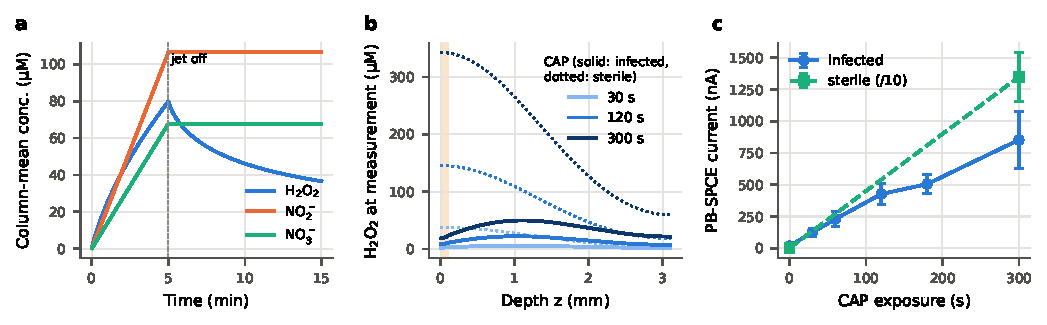
\includegraphics[width=\textwidth]{fig2_chemistry}
\caption{Plasma chemistry in the wound phantom. \textbf{a} Column-mean concentrations during a 300-s treatment and the 10-min hold. \textbf{b} H$_2$O$_2$ depth profiles at the time of measurement in infected (solid) and sterile (dotted) phantoms; the shaded band marks the biofilm. \textbf{c} Prussian-blue SPCE current (mean $\pm$ SD, $n=6$); sterile values are divided by 10.}
\label{fig:chem}
\end{figure*}

The log$_{10}$ reduction rose from $0.31\pm0.09$ at 30\,s to $2.11\pm0.37$ at 300\,s (Fig.~\ref{fig:inact}a; $F_{6,35}=99.0$, $p=1.8\times10^{-20}$). A Weibull fit in treatment time gave $b=123\pm7$\,s and $p=0.83\pm0.07$. The order of magnitude agrees with the 1--2 log reductions reported for biofilms and ex vivo skin \cite{bagheri2023,baz2023}. Survival was strongly depth-dependent: after 300\,s it rose four-fold from the surface to the base of the biofilm (Fig.~\ref{fig:inact}b). Gas flow alone produced no significant reduction (Tukey $p=1.00$ vs Control). At 30\,s the CFU reduction was not yet significant ($p=0.094$), although half of the cells were already permeabilised ($P=0.50\pm0.10$).

\begin{figure}[t]
\centering
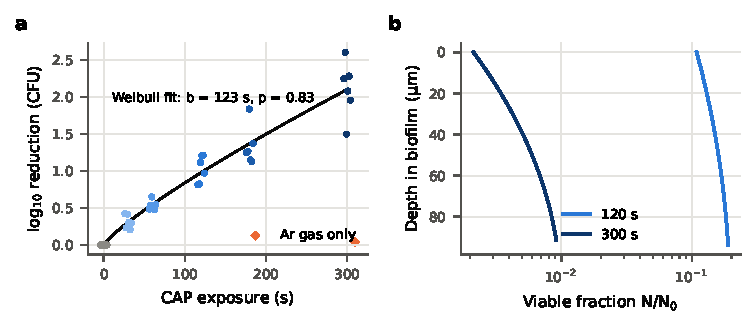
\includegraphics[width=\columnwidth]{fig3_inactivation}
\caption{Biofilm inactivation. \textbf{a} log$_{10}$ reduction of the six replicates per group with a Weibull fit in exposure time; the Ar-gas-only control is shown as diamonds. \textbf{b} Depth profile of the viable fraction for one replicate after 120\,s and 300\,s of CAP.}
\label{fig:inact}
\end{figure}

\subsection{Wideband bioimpedance}

Three regions are visible in every spectrum (Fig.~\ref{fig:spectra}a,b). Electrode polarisation dominates below about \SI{3}{\kilo\hertz}. A resistive plateau follows between \SI{10}{\kilo\hertz} and \SI{3}{\mega\hertz}. Above \SI{5}{\mega\hertz} the biofilm $\beta$-dispersion appears, superimposed on the stray capacitance. All 54 spectra passed Lin-KK with RMS residuals of $0.28\pm0.01\%$ (maximum 0.30\%), which is the noise floor. The CNLS model reached a mean reduced $\chi^2$ of $3.2\times10^{-6}$, consistent with the imposed noise, and showed no structured residuals (Fig.~\ref{fig:spectra}b inset; Fig.~\ref{fig:valid}a). After the fitted EP term is removed, the apparent permittivity of the control biofilm shows a step of about 180 units centred near \SI{17}{\mega\hertz} (Fig.~\ref{fig:spectra}c). This step shrinks progressively with CAP exposure, while the low-frequency conductivity increases (Fig.~\ref{fig:spectra}d).

\begin{figure*}[t]
\centering
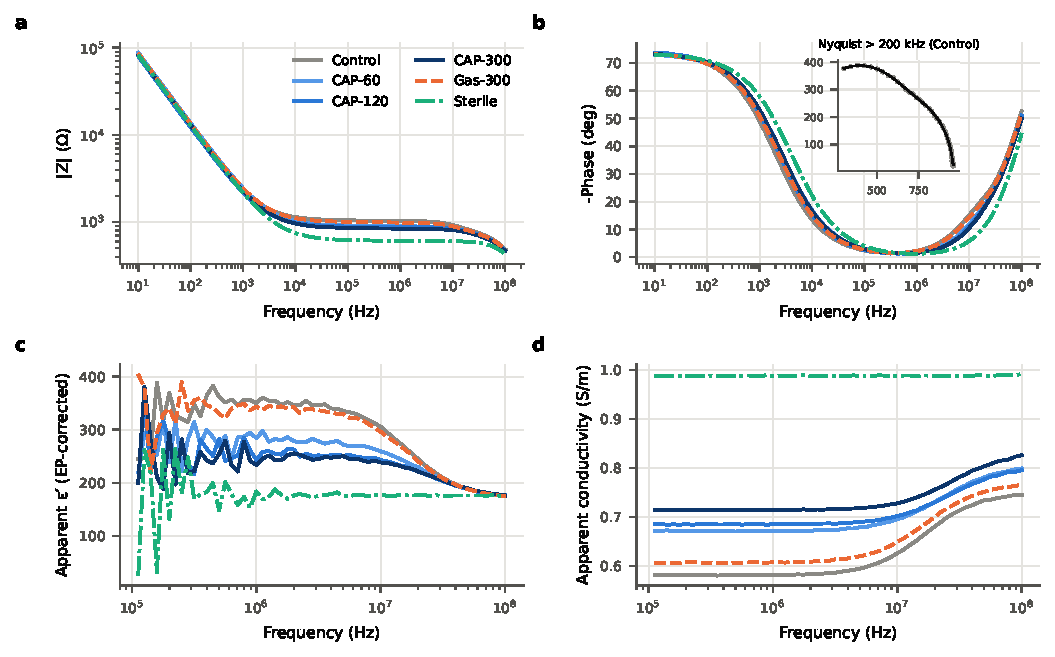
\includegraphics[width=\textwidth]{fig4_spectra}
\caption{Wideband IDE bioimpedance (means of $n=6$). \textbf{a} Impedance modulus and \textbf{b} phase; the inset shows a high-frequency Nyquist plot of one control spectrum with its CNLS fit. \textbf{c} Apparent permittivity and \textbf{d} conductivity after subtraction of each replicate's fitted electrode-polarisation CPE.}
\label{fig:spectra}
\end{figure*}

Table~\ref{tab:groups} and Fig.~\ref{fig:params} summarise the fitted parameters. The relative standard errors of $\Delta\varepsilon$ and $f_c$ were $<1.5\%$. Between Control and CAP-300, $\Delta\varepsilon$ fell by 57\% ($182\pm10 \to 78\pm2$; $\eta^2=0.953$), $f_c$ rose by 63\% ($16.6\to27.1$\,MHz; $\eta^2=0.973$), $\sigma$ rose by 23\% and $|Z|$ at 100\,kHz fell by 18\%. The rise in $f_c$ is the expected signature of shrunken, leaky cells that relax faster. $\Delta\varepsilon$ and $f_c$ already differed significantly from Control at 30\,s (Tukey $p=6.9\times10^{-10}$ and $4.7\times10^{-5}$), when the CFU difference was not significant. $\Delta\varepsilon$ was linear in the permeabilised fraction ($R^2=0.971$; Fig.~\ref{fig:params}f) and therefore saturated once $P>0.9$ (CAP-120 vs CAP-300, $p=0.87$). $f_c$ continued to separate CAP-180 from CAP-300 ($p=0.040$), because it also responds to biofilm thinning and cytoplasmic leakage. The Cole--Cole $\alpha$ stayed below 0.035: it was near zero for homogeneous populations and largest for mixed live/permeabilised populations at 30--60\,s, which makes it a qualitative marker of heterogeneity. None of the bioimpedance parameters differed between Gas-300 and Control (all $p>0.49$). This rules out drying of the phantom as a confounder at the level tested.

\begin{sidewaystable}
\caption{Ground-truth and measured quantities per group (mean $\pm$ SD, $n=6$ virtual phantoms). n.d.: not defined (no $\beta$-dispersion in cell-free phantoms).}
\label{tab:groups}
\centering
\footnotesize
\setlength{\tabcolsep}{3.5pt}
\begin{tabular}{lccccccccc}
\toprule
Quantity & Control & CAP-30 & CAP-60 & CAP-120 & CAP-180 & CAP-300 & Gas-300 & Sterile & Sterile+CAP \\
\midrule
\inputtable{tables/table_groups.tex}
\bottomrule
\end{tabular}
\end{sidewaystable}

\begin{figure*}[t]
\centering
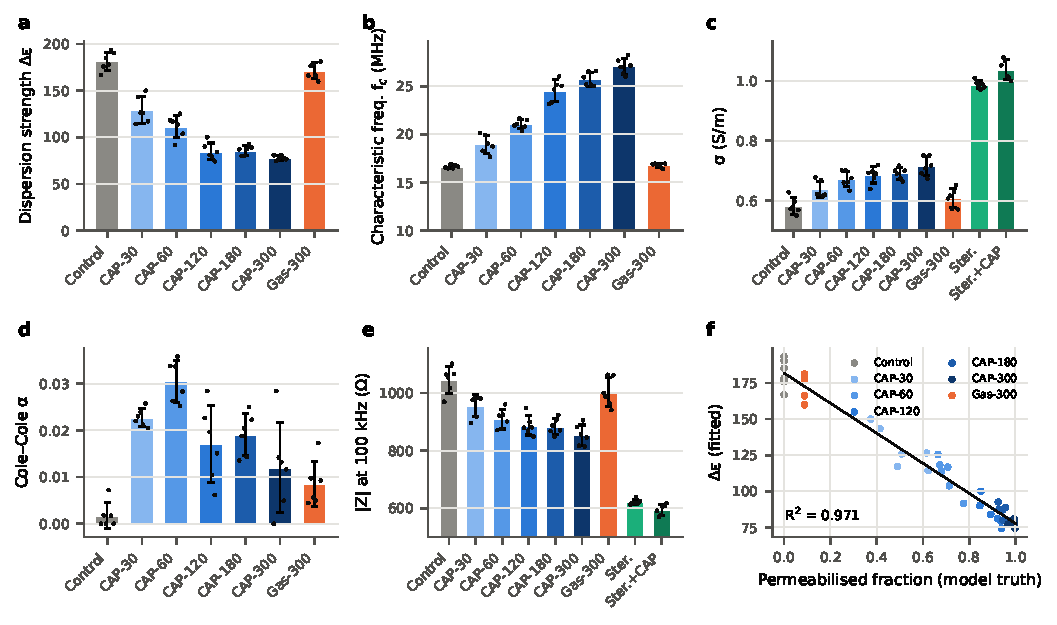
\includegraphics[width=\textwidth]{fig5_parameters}
\caption{CNLS-extracted bioimpedance parameters (bars: mean $\pm$ SD; dots: replicates). \textbf{a} $\beta$-dispersion strength, \textbf{b} characteristic frequency, \textbf{c} low-frequency conductivity, \textbf{d} Cole--Cole $\alpha$, \textbf{e} $|Z|$ at 100\,kHz. \textbf{f} Linear relation between $\Delta\varepsilon$ and the model's permeabilised fraction.}
\label{fig:params}
\end{figure*}

\paragraph{Ionic artefact in sterile phantoms.} A cell-free phantom has no $\beta$-dispersion. After 300\,s of CAP its conductivity nevertheless rose by 5.1\% ($0.988\to1.038$\,S\,m$^{-1}$; Welch $p=0.012$) and $|Z|_{100\,\mathrm{kHz}}$ fell by 4.3\% ($p=0.017$). This change comes from plasma-derived nitrite/nitrate and evaporative concentration. Buffer protonation almost cancels the conductivity added by the anions. In infected phantoms the corresponding conductivity change was 23\%, so about one fifth of the low-frequency contrast is non-biological, whereas the dispersion parameters are free of this artefact. Low-frequency conductivity or single-frequency $|Z|$ should therefore not be used alone as a marker of efficacy.

\subsection{Electrochemical characterisation}

On sterile phantoms the ferri/ferrocyanide probe behaved as a quasi-reversible couple ($\Delta E_p = 144\pm2$\,mV; $R_{ct}=0.76\pm0.03$\,k$\Omega$). The untreated biofilm blocked the electrode: $R_{ct}$ rose to $2.02\pm0.32$\,k$\Omega$ and $\Delta E_p$ to $213\pm14$\,mV (Fig.~\ref{fig:echem}). CAP progressively unblocked the electrode, decreasing $R_{ct}$ by 40\% and $\Delta E_p$ by 40\,mV at 300\,s ($F_{6,35}=12.3$ and $10.9$, both $p<10^{-6}$). Like $\Delta\varepsilon$, the electrochemical response saturated beyond 120\,s. It was also noisier ($\eta^2 \approx 0.66$--$0.68$) because it inherits the electrode-to-electrode spread of $k^0$. $R_{ct}$ was unchanged in sterile phantoms ($p=0.30$), so the faradaic channel responds to biofilm coverage and not to ionic changes. Spearman correlations with viable count were $\rho=0.80$ ($R_{ct}$), $0.78$ ($\Delta E_p$) and $-0.94$ (H$_2$O$_2$ current). The measured surface pH was uninformative ($\rho=0.10$, $p=0.55$).

\begin{figure*}[t]
\centering
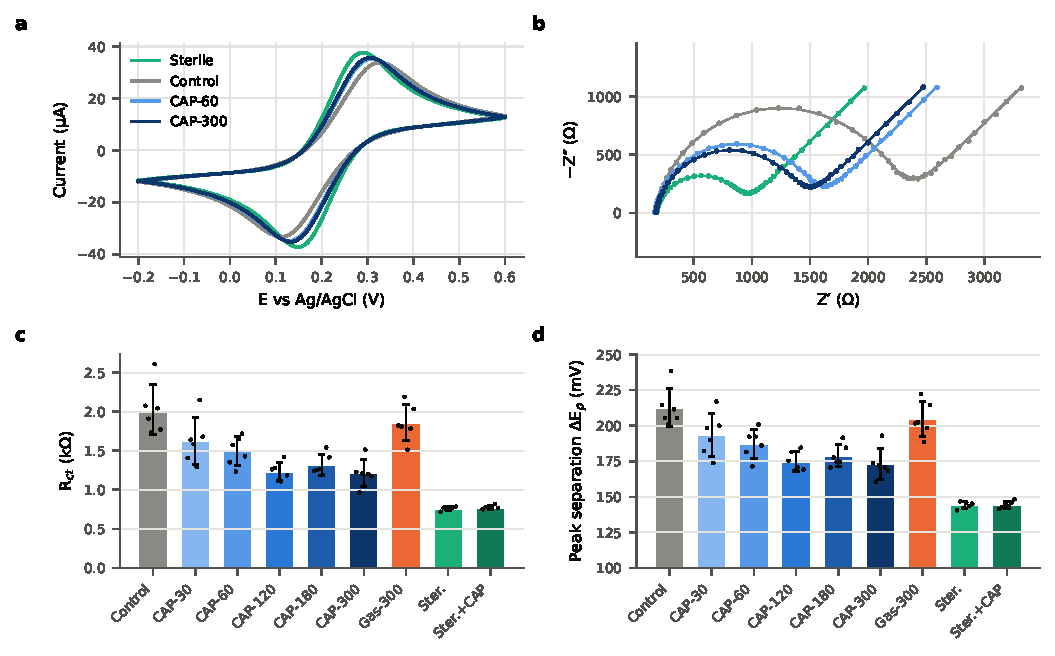
\includegraphics[width=\textwidth]{fig6_electrochem}
\caption{SPCE electrochemistry with the [Fe(CN)$_6$]$^{3-/4-}$ probe. \textbf{a} Cyclic voltammograms (50\,mV\,s$^{-1}$, second cycle). \textbf{b} Nyquist plots (symbols) with Randles fits (lines). \textbf{c} Charge-transfer resistance and \textbf{d} CV peak separation (mean $\pm$ SD, $n=6$).}
\label{fig:echem}
\end{figure*}

\begin{table}[t]
\caption{One-way ANOVA across the seven infected groups ($\mathrm{df}=6, 35$).}
\label{tab:anova}
\centering
\small
\begin{tabular}{lccc}
\toprule
Variable & $F$ & $p$ & $\eta^2$ \\
\midrule
\inputtable{tables/table_anova.tex}
\bottomrule
\end{tabular}
\end{table}

\subsection{Feature ranking and chemometric prediction}

Frequency-resolved ANOVA (Fig.~\ref{fig:ml}a) shows that the group information sits in two bands. The phase between about 1 and \SI{20}{\mega\hertz} carries most of it ($F_{\max}=67.6$ at \SI{3.5}{\mega\hertz}). The modulus plateau between 10\,kHz and 1\,MHz carries less ($F_{\max}=19.7$). The EP region below 1\,kHz is uninformative. The VIP scores of the PLS model confirm the same bands (Fig.~\ref{fig:ml}c). A nested-cross-validated, three-latent-variable PLS model predicted log$_{10}$ CFU from raw spectra with $Q^2=0.51$ and RMSECV $=0.52$ log (Fig.~\ref{fig:ml}b). Most of the error came from the 300-s group, where the dielectric contrast saturates. Among single features, $f_c$ ranked highest ($\rho=-0.95$, $p=1.3\times10^{-22}$), followed by the H$_2$O$_2$ current ($-0.94$), $\Delta\varepsilon$ ($0.92$), the 5-MHz phase ($-0.92$) and $|Z|_{100\,\mathrm{kHz}}$ ($0.85$).

\begin{figure*}[t]
\centering
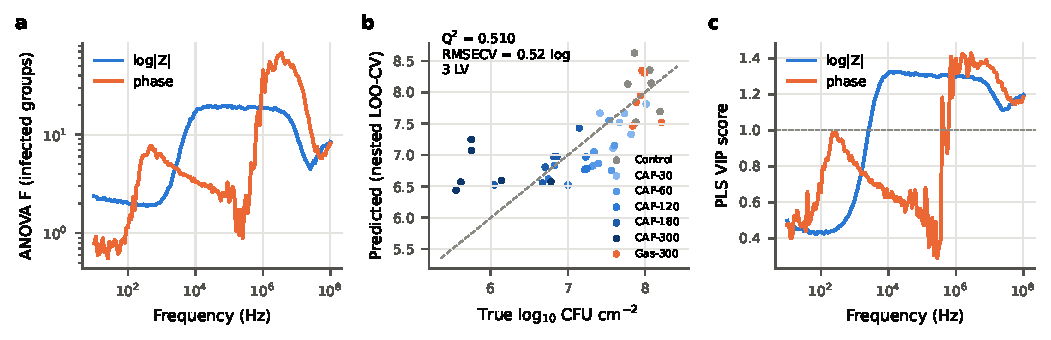
\includegraphics[width=\textwidth]{fig7_regression}
\caption{Spectral information content. \textbf{a} Frequency-resolved one-way ANOVA $F$ statistic across infected groups. \textbf{b} Nested leave-one-out predictions of log$_{10}$ CFU by PLS on raw spectra. \textbf{c} VIP scores; values above 1 mark informative variables.}
\label{fig:ml}
\end{figure*}

\subsection{Robustness}

For the main bioimpedance contrast, the relative loss of $\Delta\varepsilon$ between Control and CAP-300 was 58.4\% at baseline. It varied by less than 3 percentage points under $\pm20\%$ changes of membrane permittivity, cytoplasmic conductivity, cell fraction, biofilm thickness and IDE penetration length. It was moderately sensitive to cell radius and medium conductivity (spans of 6.4 and 5.1 points). It was most sensitive to the permeabilised fraction itself (Fig.~\ref{fig:valid}b). The contrast is therefore set mainly by membrane integrity, which is the intended target, and not by uncertain geometric or material parameters.

\begin{figure*}[t]
\centering
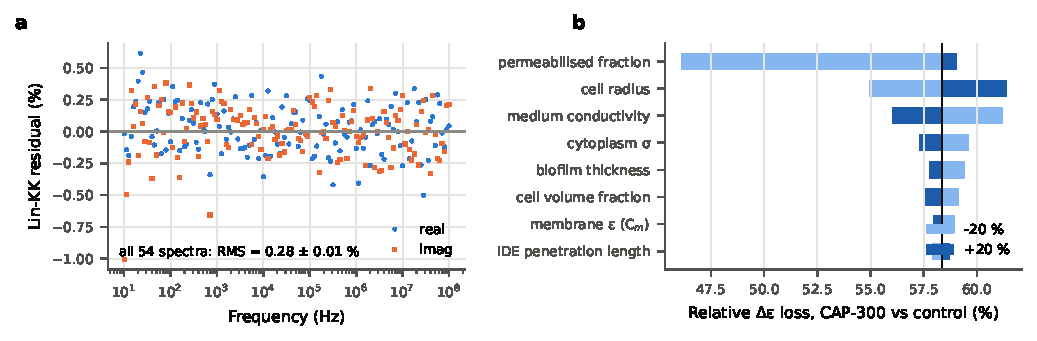
\includegraphics[width=\textwidth]{fig8_validation}
\caption{Validation and sensitivity. \textbf{a} Lin-KK residuals of a control spectrum. \textbf{b} One-at-a-time $\pm20\%$ sensitivity of the relative $\Delta\varepsilon$ loss (CAP-300 vs Control); the vertical line marks the baseline.}
\label{fig:valid}
\end{figure*}

%% ===================================================================
\section{Discussion}\label{sec:discussion}

\paragraph{A membrane-level marker that complements CFU.} In our model, the high-MHz $\beta$-dispersion measures the fraction of cells with intact envelopes, whereas colony counts measure the logarithm of the surviving fraction. The two read-outs therefore cover complementary ranges. Bioimpedance resolves early and partial damage well: it gave a significant result at 30\,s, when the CFU reduction was not yet significant. It loses resolution once more than about 90\% of the cells are permeabilised, i.e.\ beyond about one log. This behaviour follows directly from our assumption that permeabilisation equals loss of culturability ($\kappa = 1$). If membrane damage precedes cell death, as suggested for oxidative stress, the early sensitivity would increase further. If cells enter a viable-but-non-culturable state without membrane damage, it would decrease. Measuring this relation, for example with propidium-iodide staining alongside impedance, is the first experiment we recommend. The characteristic frequency extends the dynamic range because it also responds to biofilm thinning and cytoplasmic leakage. A combined $\{\Delta\varepsilon, f_c\}$ read-out, or a multivariate model, is therefore preferable to any single parameter.

\paragraph{Why the controls matter.} Two artefacts that would confound a naive experiment are separated by design. First, plasma-derived ions and evaporation shift the low-frequency conductivity even without bacteria (5\% here). Dispersion parameters, which are referenced to the high-frequency permittivity, are immune to this shift. Second, the gas flow alone could dry or cool the phantom; in our parameter range it changed no read-out. Both controls should be part of any experimental protocol. Gas-only controls, in particular, are often omitted in CAP studies \cite{maiprochnow2014}.

\paragraph{The biofilm protects itself chemically.} The 16-fold depletion of H$_2$O$_2$ in infected compared with sterile phantoms, together with the four-fold survival gradient across \SI{100}{\micro\metre}, shows that bacterial catalase and hindered diffusion explain much of the biofilm tolerance to CAP. This agrees with the strong dependence on liquid-film thickness observed experimentally \cite{hafner2018,plattfaut2021,szili2018}. It also means that H$_2$O$_2$ measured in sterile phantoms, the usual dosimetry practice, overestimates the dose that reaches cells in an infected wound. An in situ Prussian-blue sensor measures what remains in the biofilm and correlated almost as strongly with viable count as $f_c$ did. A buffered phantom kept the pH neutral, so acidified-nitrite pathways contributed nothing. Weakly buffered exudates, or plasma sources dominated by reactive nitrogen species, may behave differently and can be studied by changing two parameters of the framework.

\paragraph{Instrumentation implications.} The informative band lies above 1\,MHz, where cable parasitics and stray capacitance are largest. Validation will therefore need careful open/short/load compensation, short connections and an IDE geometry whose penetration length is comparable to the biofilm thickness. In our sensitivity analysis $\lambda$ mattered little in the range studied, which leaves room for flexible, wound-conformable electrodes. Frequencies below 1\,kHz are dominated by electrode polarisation and can be dropped, which shortens a sweep to a few seconds. This makes CAP treatment with closed-loop impedance feedback technically plausible.

\paragraph{Limitations.} This is a computational study. All quantitative results depend on assumed parameters, and the model needs experimental calibration before its numbers can be compared with any device. Specifically: (i) plasma fluxes are constant, and short-lived species (OH, O$_3$, ONOO$^-$), UV and electric-field effects are lumped into the long-lived H$_2$O$_2$/HNO$_2$ dose; (ii) the IDE is modelled by an exponential-sensitivity, parallel-path approximation rather than a full field solution; (iii) the bacteria are single-shell spheres, without explicit cell-wall or EPS charge relaxation (the $\alpha$-dispersion) and without host cells; (iv) H$_2$O$_2$ consumption does not feed back on the evolving viable density; and (v) temperature is assumed to be equilibrated at measurement. Noise and variability levels were chosen to be representative, not measured. The code nevertheless analyses measured spectra in a standard CSV format without modification, so the same CNLS, Lin-KK and statistical pipeline can be applied directly to experimental data.

%% ===================================================================
\section{Conclusions}\label{sec:conclusion}

We presented an open multiphysics framework that links CAP chemistry, depth-resolved biofilm inactivation and two electrical read-out channels in an infected wound phantom. Within the model, three findings stand out. First, the high-MHz $\beta$-dispersion ($\Delta\varepsilon$ and especially $f_c$) is a Kramers--Kronig-consistent, label-free marker of CAP-induced membrane damage that responds earlier than colony counts. Second, gas-only and sterile controls are necessary to separate biological effects from ionic and evaporative artefacts. Third, an in situ H$_2$O$_2$ sensor together with faradaic EIS adds direct dosimetry and biofilm-coverage information. These results provide testable hypotheses, target frequency bands and sensitivity bounds for the experimental validation that must follow.

\backmatter

\bmhead{Acknowledgements}
The author thanks the management and the Department of Electronics and Communication Engineering, Velalar College of Engineering and Technology, for support.

\section*{Declarations}

\begin{itemize}
\item \textbf{Funding:} No external funding was received for this work. [Author to update if applicable.]
\item \textbf{Conflict of interest:} The author declares no competing interests.
\item \textbf{Ethics approval and consent to participate:} Not applicable; this is a purely computational study with no human or animal participants and no biological material.
\item \textbf{Consent for publication:} Not applicable.
\item \textbf{Data availability:} All simulated data (per-sample tables, group summaries, statistical outputs) are generated by the accompanying code and are included in the repository (\texttt{results/}).
\item \textbf{Code availability:} The complete framework (\texttt{capwound} Python package, analysis script and unit tests) is openly available in the author's repository; a DOI-versioned archive will be created on acceptance.
\item \textbf{Use of AI tools:} An AI assistant (Claude, Anthropic) was used to help write the simulation code, run the analyses and draft the manuscript text. The author reviewed, verified and takes full responsibility for all content, including model assumptions, results and references.
\item \textbf{Author contribution:} M.N.A.: conceptualisation, methodology, software, formal analysis, writing (original draft, review and editing).
\end{itemize}

\bibliography{references}
\IfFileExists{sn-jnl.cls}{}{\bibliographystyle{unsrtnat}}

\end{document}
